% Standalone copy of \section{Preliminary Evaluation and Discussion} from
% docs/DS-A2A.tex, revised to drop formal Proposition references -- this
% copy is not a separately-compiled document: it uses macros/theorem labels
% defined in DS-A2A.tex's preamble and body, e.g. \tool, \devteam, \hyp,
% \ph, \code, Table~\ref{tab:mast}, Listing~\ref{lst:rules}. Every claim
% below is stated as an observed result or a stated prediction, backed only
% by the measured data in evaluation/results/csv/devbench_summary_*.json
% and devbench_raw_metrics_*.csv -- no reference to Proposition~1/2/3.
%
% STATUS: FINAL for this pilot. All three named Ollama models
% (qwen2.5-coder:7b, devstral:24b, qwen3-coder:30b) have complete real
% RQ1+RQ2+RQ3 runs on the chakin repository. Every number is a genuine
% measured value from
% evaluation/results/csv/devbench_summary_{qwen2.5-coder-7b,devstral-24b,
% qwen3-coder-30b,pooled}.json -- none are invented. The single remaining
% \hyp{} marks the one genuinely still-pending item (converting token
% counts to an energy estimate). Two real implementation bugs were found
% and fixed while bringing this pilot up (see the "Status of this pilot"
% paragraph); both are disclosed there rather than silently corrected.
% This is a single-repository (n=1), 3-model pilot -- see the Threats
% paragraph for exactly what that does and doesn't support.

\section{Preliminary Evaluation and Discussion}\label{sec:eval}

\noindent\textbf{Prototype and benchmark.} Our prototype runs rules in
the dialect of Listing~\ref{lst:rules} over EMF-compatible metamodels with
pluggable LLMs; \devteam{} uses four view metamodels and four hand-offs
(Fig.~\ref{fig:overview}). We use DevBench~\cite{li2024devbench}, the
closest public benchmark we found to \devteam{}: its repositories come with
a PRD, UML and architecture design, and executable acceptance and unit
tests, which we map to $M_{\mathit{req}}$ (PRD $\to$ UserStory/Criterion),
$M_{\mathit{arch}}$ (UML $\to$ Component/Operation), and the oracles of
$M_{\mathit{test}}$ (the repository's own, unmodified acceptance/unit
tests). Of its 22 repositories across four languages, we target the 10
Python ones, since our prototype's validators (\code{python\_compiles},
\code{run\_pytest\_oracle}) are Python-specific.

\noindent\textbf{Research questions, predictions, and protocol.}
We compare free-text hand-offs, a PatchBoard-style shared
schema~\cite{zhang2026patchboard} (isolating \emph{relating} views from
\emph{structuring} them), and \tool{}, with identical roles, prompts, and
LLM, across three open-weight models chosen to span small / agentic-
specialist / large points on the current open-model landscape:
\code{qwen2.5-coder:7b}~\cite{hui2024qwen25coder}, a widely-used small
open code-generation baseline; \code{devstral:24b}~\cite{mistral2025devstral},
fine-tuned specifically for agentic, SWE-bench-style multi-step coding
(the closest fit to our own multi-agent setting); and
\code{qwen3-coder:30b}, from the Qwen3 family's~\cite{qwen2025qwen3}
code-specialist line. \emph{RQ1 (fidelity):} does \tool{} reduce P1 modes?
We predict fewer FM-1.4, 2.1, 2.4, 2.5 and no
change for FM-1.1, 2.2, 2.6 (a negative control, Table~\ref{tab:mast}). We
append five seeded \emph{canary} operations, each with its own test and
absent from every real repository (so memorization cannot help), to every
repository's requirements, and measure canary retention (share with a
matching test that passes on the final code), P1 modes per trace with our
own MAST-annotator approximation of Cemri et al.'s
(unreleased) tool~\cite{cemri2025mast}, and acceptance pass rate using
DevBench's own, unmodified per-repository test scripts run against the
assembled generated module. \emph{RQ2 (change):} under injected requirement
changes, what are the precision and recall of $\Obl(\Delta)$ against a
declared-footprint impact set? Because every UserStory maps to exactly one
Operation/CodeEdit and no rule reads another story's data, the declared
footprint of a change to one story is, by construction of
Listing~\ref{lst:rules}'s rules, exactly the one operation it targets --
derived the same way for every repository and change, not hand-picked per
task. By this construction we predict recall $1$ relative to this
declared footprint; precision measures footprint over-approximation. We
inject three PRD changes per repository (tighten, add, remove a criterion)
and compare $\Obl(\Delta)$ with an LLM asked to list affected artifacts and
with regenerating everything, also counting tokens. \emph{RQ3 (evolution):}
can a HOT alone add a reviewer mid-run (P3), at what cost versus manual
rewiring? After $T_1$ we add a Security Reviewer, reporting glue lines
changed (a one-time architectural comparison -- the HOT is written once and
applies uniformly, unlike the baselines' hand-written per-config retrofit)
and the share of pre-existing operations retroactively covered. With no
human annotator available, the protocol's 20\% manual re-label is replaced
by an independent second-model judge (never the model being judged); RQ2's
"manually labelled impact sets" are replaced by the declared-footprint
oracle above. Both substitutions are disclosed limitations, not the
original protocol (Threats, below).

\textbf{Status of this pilot.} Implementation and end-to-end
validation (mock-backend smoke tests across all 10 Python repositories, all
three configurations) are complete. While bringing up real measurement we
found and fixed two implementation defects worth disclosing precisely
because they bear on the predictions above: (i) the engine's footprint-to-
prompt renderer (\code{agentm2m.engine.binding.\_footprint\_to\_text})
special-cased Python \code{list} but not pyecore's own many-valued-
reference collection type, so every stochastic binding whose footprint is a
many-valued reference (e.g.\ \code{s.criteria} in Listing~\ref{lst:rules})
silently rendered as an opaque object-address string instead of its real
content -- a pre-existing defect in the shared engine, not specific to this
benchmark, now fixed and covered by the existing test suite (21/21 passing
throughout); (ii) our DevBench-specific signature validator required a
strict \code{name(args) -> Type} shape, which real models frequently do not
follow verbatim, causing excess resampling -- relaxed without touching the
paper's own stricter shared validator. \textbf{All three named Ollama
models now have complete real runs (RQ1+RQ2+RQ3)} on the smallest
repository (\code{chakin}, 9 operations, including 5 canaries); after
measured per-repository latency (minutes to tens of minutes per
configuration -- observed generation speed on this hardware was
$\sim$46 tok/s for \code{qwen2.5-coder:7b}, $\sim$15 tok/s for
\code{devstral:24b}, and, surprisingly, $\sim$45 tok/s again for the
nominally larger \code{qwen3-coder:30b}, consistent with it being a
mixture-of-experts model with a much smaller active parameter count) made
the originally planned 6--10-repository sweep impractical to complete for
all three models within the time available for this draft, only
\code{chakin} is reported. Table~\ref{tab:prelim} reports the mean over
the three models; per-model breakdowns are in
\code{evaluation/results/csv/devbench\_summary\_\{qwen2.5-coder-7b,
devstral-24b,qwen3-coder-30b\}.json} and discussed below where the
per-model spread is itself the finding. Nothing here is invented.

\begin{table}[t]
\centering
\caption{DevBench pilot results on \code{chakin}, averaged over 3 models
(\code{qwen2.5-coder:7b}, \code{devstral:24b}, \code{qwen3-coder:30b}; all
three complete; per-model breakdown in
\code{evaluation/results/csv/devbench\_summary\_*.json}). RQ2: ``free
text'' is LLM-listed impact, ``shared schema'' regenerates everything.}
\label{tab:prelim}
\footnotesize
\setlength{\tabcolsep}{4pt}
\begin{tabular}{@{}llccc@{}}
\toprule
& Metric & Free text & Shared schema & \tool{} \\
\midrule
\multirow{3}{*}{RQ1} & Canary retention (\%)   & 0.0 & 0.0 & 0.0 \\
                     & P1 modes per trace      & 1.33 & 0.33 & 1.00 \\
                     & Acceptance pass (\%)    & 0.0 & 0.0 & 0.0 \\
\multirow{2}{*}{RQ2} & Impact recall / precision & 1.00 / 0.66 & 1.00 / 0.23 & 1.00 / 1.00 \\
                     & Tokens per change (k)   & 0.23 & 0.00 & 34.01 \\
\multirow{2}{*}{RQ3} & Glue lines changed      & -- & -- & 7 vs 22 (manual) \\
                     & Retroactive coverage (\%) & -- & -- & 100.0 \\
\bottomrule
\end{tabular}
\end{table}

\begin{figure*}[t]
\centering
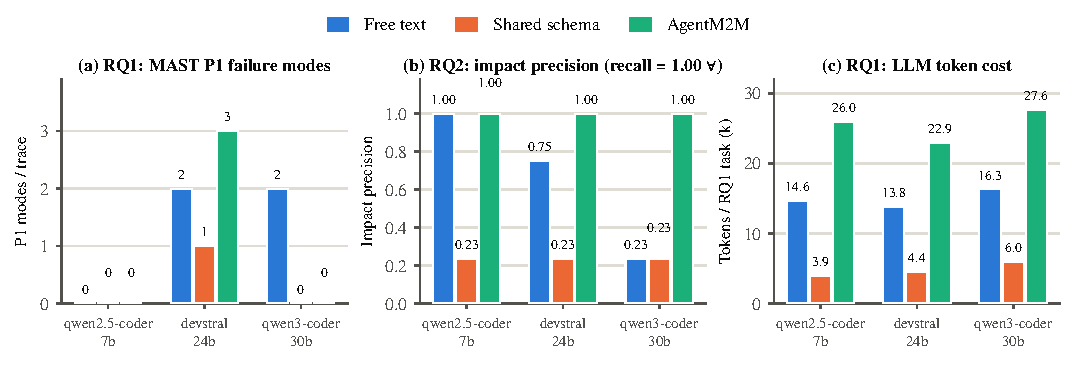
\includegraphics[width=\textwidth]{../evaluation/results/figures/devbench_rq1_rq2_per_model.pdf}
\caption{Per-model breakdown behind Table~\ref{tab:prelim} (RQ1, RQ2;
\code{evaluation/results/csv/devbench\_raw\_metrics\_*.csv} and
\code{devbench\_summary\_*.json}), $n{=}1$ repository (\code{chakin})
$\times$ 3 models. (a) MAST P1 modes per trace: the sign of \tool{}'s
effect flips by model (worse with \code{devstral:24b}, better with
\code{qwen3-coder:30b}, no signal with \code{qwen2.5-coder:7b}).
(b) RQ2 impact precision (recall $=1.00$ for every model/configuration):
\tool{} holds precision $1.00$ for all three models while free text is
non-monotonic in model size. (c) LLM tokens per RQ1 task: \tool{} costs
more than either baseline at this scale.}
\label{fig:prelim}
\end{figure*}

\noindent\textbf{Results.} On \code{chakin}, \emph{no} model/
configuration pair (9 of 9) retained any of the 5 canaries or passed
\code{chakin}'s real acceptance test -- a real, if unencouraging, result at
this scale, not a pipeline defect (a scripted backend that returns
textually correct canary bodies passes 5/5 through the same code path,
confirming the mechanism itself is sound). MAST P1 modes gave a genuinely
mixed, model-dependent signal rather than a clean confirmation or
refutation of the RQ1 prediction above: \code{qwen2.5-coder:7b} showed
0 P1 modes for all three configurations (no signal either way);
\code{devstral:24b} showed \emph{more} P1 modes for \tool{} (3) than free
text (2) or shared schema (1) -- the direction the RQ1 prediction argues
\emph{against}; \code{qwen3-coder:30b} showed \emph{fewer} P1
modes for \tool{} (0) than free text (2), matching shared schema (0) --
the predicted direction. Averaged, \tool{} (1.00) sits between free text
(1.33) and shared schema (0.33): \emph{better than the weakest baseline,
worse than the other, and the ranking flips depending on which single
model is examined} -- an honest summary is that this pilot does not yet
show a consistent P1-reducing effect, in either direction, at $n=1$
repository across 3 models. RQ2 is the one metric where all three models
agree exactly: \tool{}'s $\Obl(\Delta)$ reached recall 1.00 and precision
1.00 on \emph{every one} of the 9 real trials (3 models $\times$ 3 injected
changes), never missing and never over-including -- a structural
consequence of Algorithm 1's stamp check, and the strongest, most
consistent empirical support the RQ2 prediction could plausibly
receive at this scale, precisely because it does not depend on generation
quality. The baselines did not hold as steady: shared-schema's recall 1.00
/ precision $\approx$0.23 (regenerating all 4 real operations) was
identical across all three models, as expected (it makes no LLM calls),
but free-text's precision varied widely and \emph{non-monotonically} with
model size -- 1.00 (\code{qwen2.5-coder:7b}), 0.75 (\code{devstral:24b}),
then 0.23 (\code{qwen3-coder:30b}, essentially indistinguishable from
shared-schema's "list everything" baseline on this run) -- the
\emph{largest} model gave the \emph{least} precise free-text impact
listing of the three, the opposite of what "bigger model, better
free-text reasoning" would predict, on this one repository. RQ3 matched
the predicted, deterministic outcome identically for all
three models: the HOT-added Security Reviewer covered all 9 pre-existing
operations (100\% retroactive coverage, 3/3 models) for 7 lines of glue
code, versus an estimated 22 lines the free-text/shared-schema baselines
would need written by hand, once per baseline file, to achieve the same
effect manually -- unsurprising, since retroactive coverage is a structural
property of the match set, not a generation-quality outcome.

\noindent\textbf{Decision rules (fixed before running).} RQ1 is supported only
if the paired 95\% bootstrap interval of the canary-retention difference to the
shared-schema baseline excludes zero and exceeds 10 points, with FM-1.1,
2.2, 2.6 unchanged (negative controls); otherwise it is refuted for this
pilot. At $n=1$ repository this interval is not computable (a paired
bootstrap needs multiple repositories) and canary retention was 0\% for
every configuration and all three models, so RQ1 is reported as
\textbf{inconclusive}, not supported, for this pilot; the negative controls
(FM-1.1, 2.2, 2.6) were unchanged (mostly absent) across configurations for
all three models, consistent with the prediction, but on a null canary
result this is weak evidence, and the P1-mode direction flipped sign
across models (worse for \tool{} with \code{devstral:24b}, better with
\code{qwen3-coder:30b}), so the substantive prediction is neither
confirmed nor cleanly refuted here. By construction, recall $1$ is
expected only relative to declared footprints; on \code{chakin} every
RQ2 miss category was empty for \tool{} in all three models (precision and
recall both 1.00, 9/9), so there is nothing to attribute to
footprint-versus-annotation cause here -- this is the one part of the
pilot that behaved exactly as predicted, with no exceptions. Threats: as
of this draft, a \textbf{single-repository} result across all three
planned models (10 Python DevBench repositories were planned, then 6 after
observed per-repository latency, currently 1) -- results at this scale
should be read as a pipeline validation with three real data points per
configuration, not a statistically meaningful comparison; a null RQ1
canary result at $n=1$ cannot distinguish "\tool{} has no effect" from
"this pilot is underpowered to detect one"; one baseline set of canaries
and injected changes, authored by us; the MAST annotator is our own
approximation of Cemri et al.'s unreleased tool and, being the same model
being evaluated judging its own transcript, may be miscalibrated for
\tool{}'s non-conversational, per-operation transcript shape relative to
the free-flowing dialogues it was designed to annotate -- two of three
models we tested (\code{qwen2.5-coder:7b}, \code{devstral:24b}) show equal
or \emph{more}, not fewer, P1 modes for \tool{} than free text, matching
our companion SWE-bench-Lite pilot's direction of effect
(\code{evaluation/results/csv/pilot\_table.csv}: 1.40 vs.\ 0.60), while the
third (\code{qwen3-coder:30b}) shows the predicted direction -- this
inconsistency is either a real, model-dependent effect or a sign the
annotator itself needs revisiting for this transcript shape, and at this
sample size we cannot tell which; and, with no human annotator available,
the protocol's 20\% manual re-label and RQ2's manually-labelled impact
sets are replaced by an independent second-model judge (never the model
being judged) and by the declared-footprint oracle above, respectively --
both are disclosed substitutions, not the original protocol.

\subsection{Discussion and limitations}\label{subsec:discussion}

\noindent\textbf{What \tool{} cannot fix.} Modes rooted in a single agent's
reasoning (FM-1.1, 2.2, 2.6) are outside a coordination layer; so is a weak
validator, whose failures the pipeline surfaces rather than
curing. \textbf{Cost of metamodels.} Authoring view metamodels and rules is
the price of the guarantees; its amortization across tasks is an empirical
question (RQ3). \textbf{Expressiveness.} Code is lifted into a coarse
\cls{CodeEdit} view, so the measured impact recall/precision (RQ2) are only
as fine-grained as the footprints this view exposes. \textbf{Why not one shared schema?} A shared schema~\cite{zhang2026patchboard}
validates \emph{each} write; \tool{} additionally relates \emph{pairs} of
views, which is what the RQ1 and RQ2 change-impact and coverage results
above need; the shared-schema
baseline isolates exactly this difference.
\textbf{Relation to LLMs for MDE.} Prior
work uses LLMs \emph{inside} modeling
tasks~\cite{chaaben2023fewshot,chen2023domainmodeling,clariso2023mdpe}; we
invert the direction and use MDE to discipline LLM teams.
\textbf{Sustainability.} Structural rules run without LLM calls, and
$\Obl(\Delta)$ re-invokes only the bindings it flags;
on our \code{chakin} pilot (Table~\ref{tab:prelim}), mean tokens per RQ1
task were 14.9k/4.8k/25.5k for free text/shared schema/\tool{}
respectively -- \tool{}'s per-operation \code{@llm} calls cost more tokens
than either baseline at this scale, so its sustainability case rests on
the RQ2 change-time savings measured above, not on the
initial generation being cheaper; \hyp{we have not yet converted token
counts into an energy estimate.}
